\section*{Problem 1}
\subsection*{Part a}
\eq{
\rho &= \frac{1}{2}(I + \Vec{r}\cdot\Vec{\sigma})\\
&= \frac{1}{2}(I + r_x \sigma_x + r_y \sigma_y + r_z \sigma_z)\\
&= \frac{1}{2}(\begin{pmatrix}
    1 & 0\\
    0 & 1
\end{pmatrix} + \begin{pmatrix}
0 & r_x\\
r_x & 0
\end{pmatrix} + \begin{pmatrix}
    0 & -ir_y \\
    ir_y & 0
\end{pmatrix} + \begin{pmatrix}
    r_z & 0\\
    0 & -r_z
\end{pmatrix})\\
&= \frac{1}{2}\begin{pmatrix}
    1 + r_z & r_x -ir_y\\
    r_x + ir_y & 1 - r_z
\end{pmatrix}
}
\subsection*{Part b}
\eq{
[\sigma_x] &= tr(\rho \sigma_x)\\
&= tr(\frac{1}{2}\begin{pmatrix}
    r_x - ir_y & 1 + r_z\\
    1- r_z & r_x + ir_y
\end{pmatrix})\\
&= r_x
}
\subsection*{Part c}
\eq{
[\sigma_z] &= tr(\rho \sigma_z)\\
&= tr(\frac{1}{2}\begin{pmatrix}
    1 + r_z & ir_y - r_x\\
    r_x + ir_y & r_z - 1
\end{pmatrix})\\
&= r_z
}

\pagebreak
\section*{Problem 2}
\subsection*{Part a}
We are given that
\eq{
[\sigma_x] &= r_x = 1\\
[\sigma_y] &= r_y = 0\\
[\sigma_z] &= r_z = 0
}
So the density matrix is
\eq{
\rho &= \frac{1}{2}(I + \sigma_x)
}
\subsection*{Part b}
$\rho$ is a pure state since it can be written as $\ket{\psi}\bra{\psi}$, where $\ket{\psi}$ is a pure state
\eq{
\ket{\psi} &= \frac{1}{\sqrt{2}}(\ket{0} + \ket{1})\\
\ket{\psi}\bra{\psi} &= \frac{1}{2}\begin{pmatrix}
    1 & 1\\
    1 & 1
\end{pmatrix}\\
&= \rho
}
\subsection*{Part c}
Both of the vectors point in the same direction so they overlap on the Bloch sphere.
\begin{figure}[H]
    \centering
    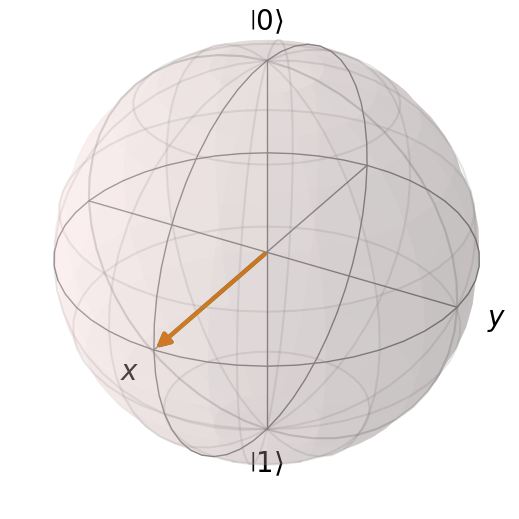
\includegraphics[width=0.75\linewidth]{Resources//245//Homework 9/245 Homework 9 Problem 2c.png}
    \label{fig:enter-label}
\end{figure}

\subsection*{Part d}
Now we are given
\eq{
[\sigma_x] &= r_x = 0.7\\
[\sigma_y] &= r_y = 0\\
[\sigma_z] &= r_z = 0
}
So the density matrix is
\eq{
\rho &= \frac{1}{2}(I + 0.7\sigma_x)
}
\subsection*{Part e}
This is not a pure state since
\eq{
\rho^2 &= \frac{1}{4}\begin{pmatrix}
    1 & 0.7\\
    0.7 & 1
\end{pmatrix}^2\\
&= \frac{1}{4}\begin{pmatrix}
    1 + 0.7^2 & 1.4\\
    1.4 & 1 + 0.7^2
\end{pmatrix}\\
&= \frac{1}{2}\begin{pmatrix}
    0.745 & 0.7\\
    0.7 & 0.745
\end{pmatrix}\\
&\neq \rho
}
\subsection*{Part f}
The vectors all point in the same direction on the Bloch sphere, however, the vector from part d has a length less than one.
\begin{figure}[H]
    \centering
    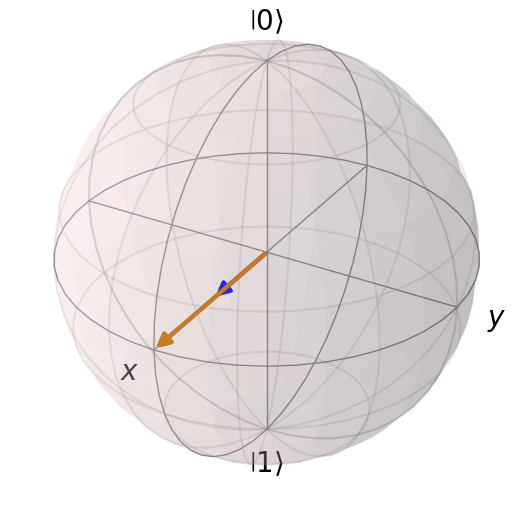
\includegraphics[width=0.75\linewidth]{Resources//245//Homework 9/245 Homework 9 Problem 2f.png}
    \label{fig:enter-label}
\end{figure}

\pagebreak
\section*{Problem 3}
\subsection*{Part a}
The density matrix is
\eq{
\rho &= \frac{1}{2}(\ket{1,0,n}+\ket{0,1,n})(\bra{1,0,n} + \bra{0,1,n})
}
\subsection*{Part b}
Tracing out the QHO terms, we get
\eq{
\rho_{S_1} &= \frac{1}{2}(\ket{1,0}+\ket{0,1})(\bra{1,0} + \bra{0,1})\\
\rho_{S_1}^2 &= \frac{1}{4}(\ket{1,0}+\ket{0,1})2(\bra{1,0} + \bra{0,1})\\
&= \rho_{S_1}
}
So this is a pure state.
\subsection*{Part c}
Now suppose
\eq{
\ket{\psi} &= a(\ket{1,0,n}+\ket{0,1,n})+b\ket{0,0,n+1}
}
Then the density matrix is
\eq{
\rho &= (a(\ket{1,0,n}+\ket{0,1,n})+b\ket{0,0,n+1})\\
&(a(\bra{1,0,n}+\bra{0,1,n})+b\bra{0,0,n+1})
}
\subsection*{Part d}
The reduced density matrix is then
\eq{
\rho_{S_2} &= |a|^22\rho_{S_1}+|b|^2\ket{0,0}\bra{0,0}\\
\rho_{S_2}^2 &= |a|^44\rho_{S_1}+|b|^4\ket{0,0}\bra{0,0}\\
}
If $|b|^2=1$ and $|a|^2 = \frac{1}{\sqrt{2}}$then this is a pure state.
\pagebreak
\section*{Problem 4}
\subsection*{Part a}
The Kraus operators are
\eq{
K_0 &= \braket{e_0 | U | e_0}\\
&= \sqrt{1-p}\braket{e_0|e_0}+\sqrt{p}X_S \otimes \braket{e_0 | G_E | e_0}\\
&= \sqrt{1-p}I_S
}
Then for some $j \neq 0$
\eq{
K_j &= \braket{e_j | U | e_0}\\
&= \sqrt{1-p}\braket{e_j|e_0}+\sqrt{p}X_S \otimes \braket{e_j | G_E | e_0}\\
&= \sqrt{p}X_S
}
and for every other $k \neq j \lor 0$
\eq{
K_k &= 0
}

\subsection*{Part b}
Assuming the system originally started in state $\ket{\psi} = \ket{0}$
\eq{
\hat{\rho}(t) &= \sum_k K_k\ket{0}\bra{0}K_k^\dag\\
&= (1-p)\ket{0}\bra{0}+p\ket{1}\bra{1}
}
\subsection*{Part c}
Assuming the system orginally started in state $\ket{\psi} = \frac{1}{\sqrt{2}}(\ket{0}+\ket{1})$
\eq{
\hat{\rho}(t) &= \frac{1}{2}\sum_k K_k(\ket{0}+\ket{1})(\bra{0}+\bra{1})K_k^\dag\\
&= \frac{1-p}{2}\ket{\psi}\bra{\psi} + \frac{p}{2}\ket{\psi}\bra{\psi}\\
&= \frac{1}{2}\ket{\psi}\bra{\psi}
}
\pagebreak
\section*{Problem 5}
\subsection*{Part a}
Results of mesolve without any collapse operators.
\begin{figure}[H]
    \centering
    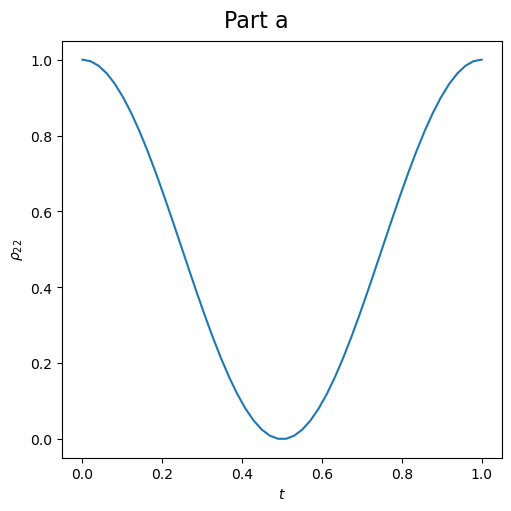
\includegraphics[width=0.75\linewidth]{Resources//245//Homework 9/245 Homework 9 Problem 5a.png}
    \label{fig:enter-label}
\end{figure}

\subsection*{Part b}
Results of mesolve simulation with varying collapse operators.
\begin{figure}[H]
    \centering
    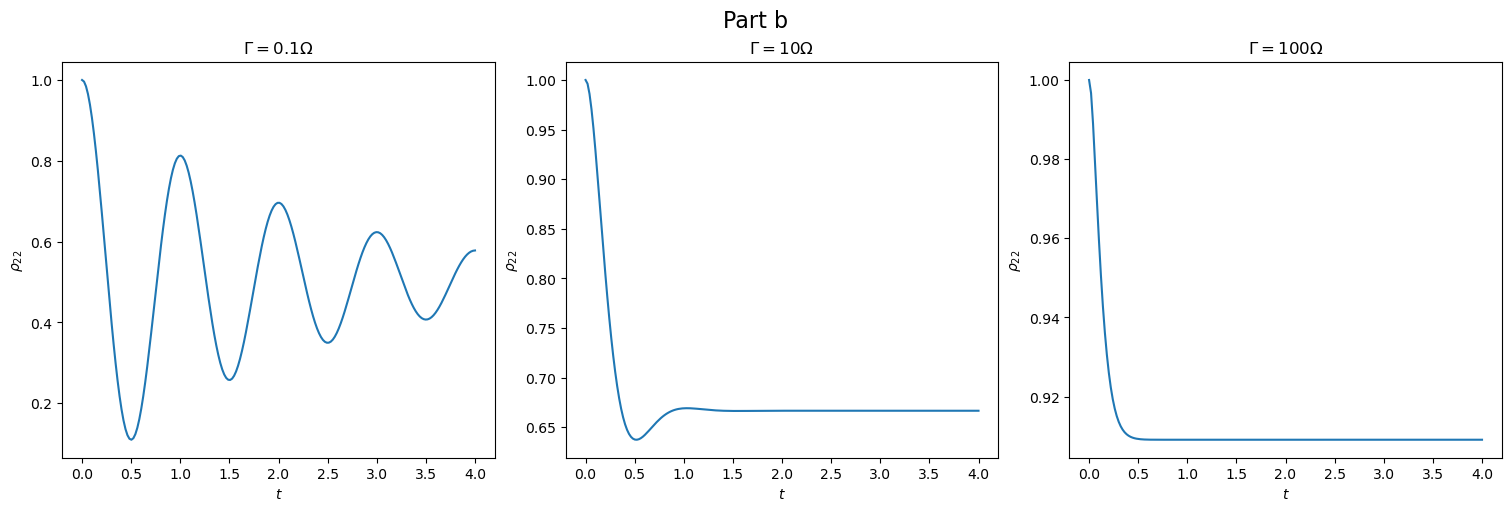
\includegraphics[width=1\linewidth]{Resources//245//Homework 9/245 Homework 9 Problem 5b.png}
    \label{fig:enter-label}
\end{figure}
\subsection*{Part c}
Results of mcsolve simulation for number of trajectories $1, 10, 100$ and varying $\Gamma$.
\begin{figure}[H]
    \centering
    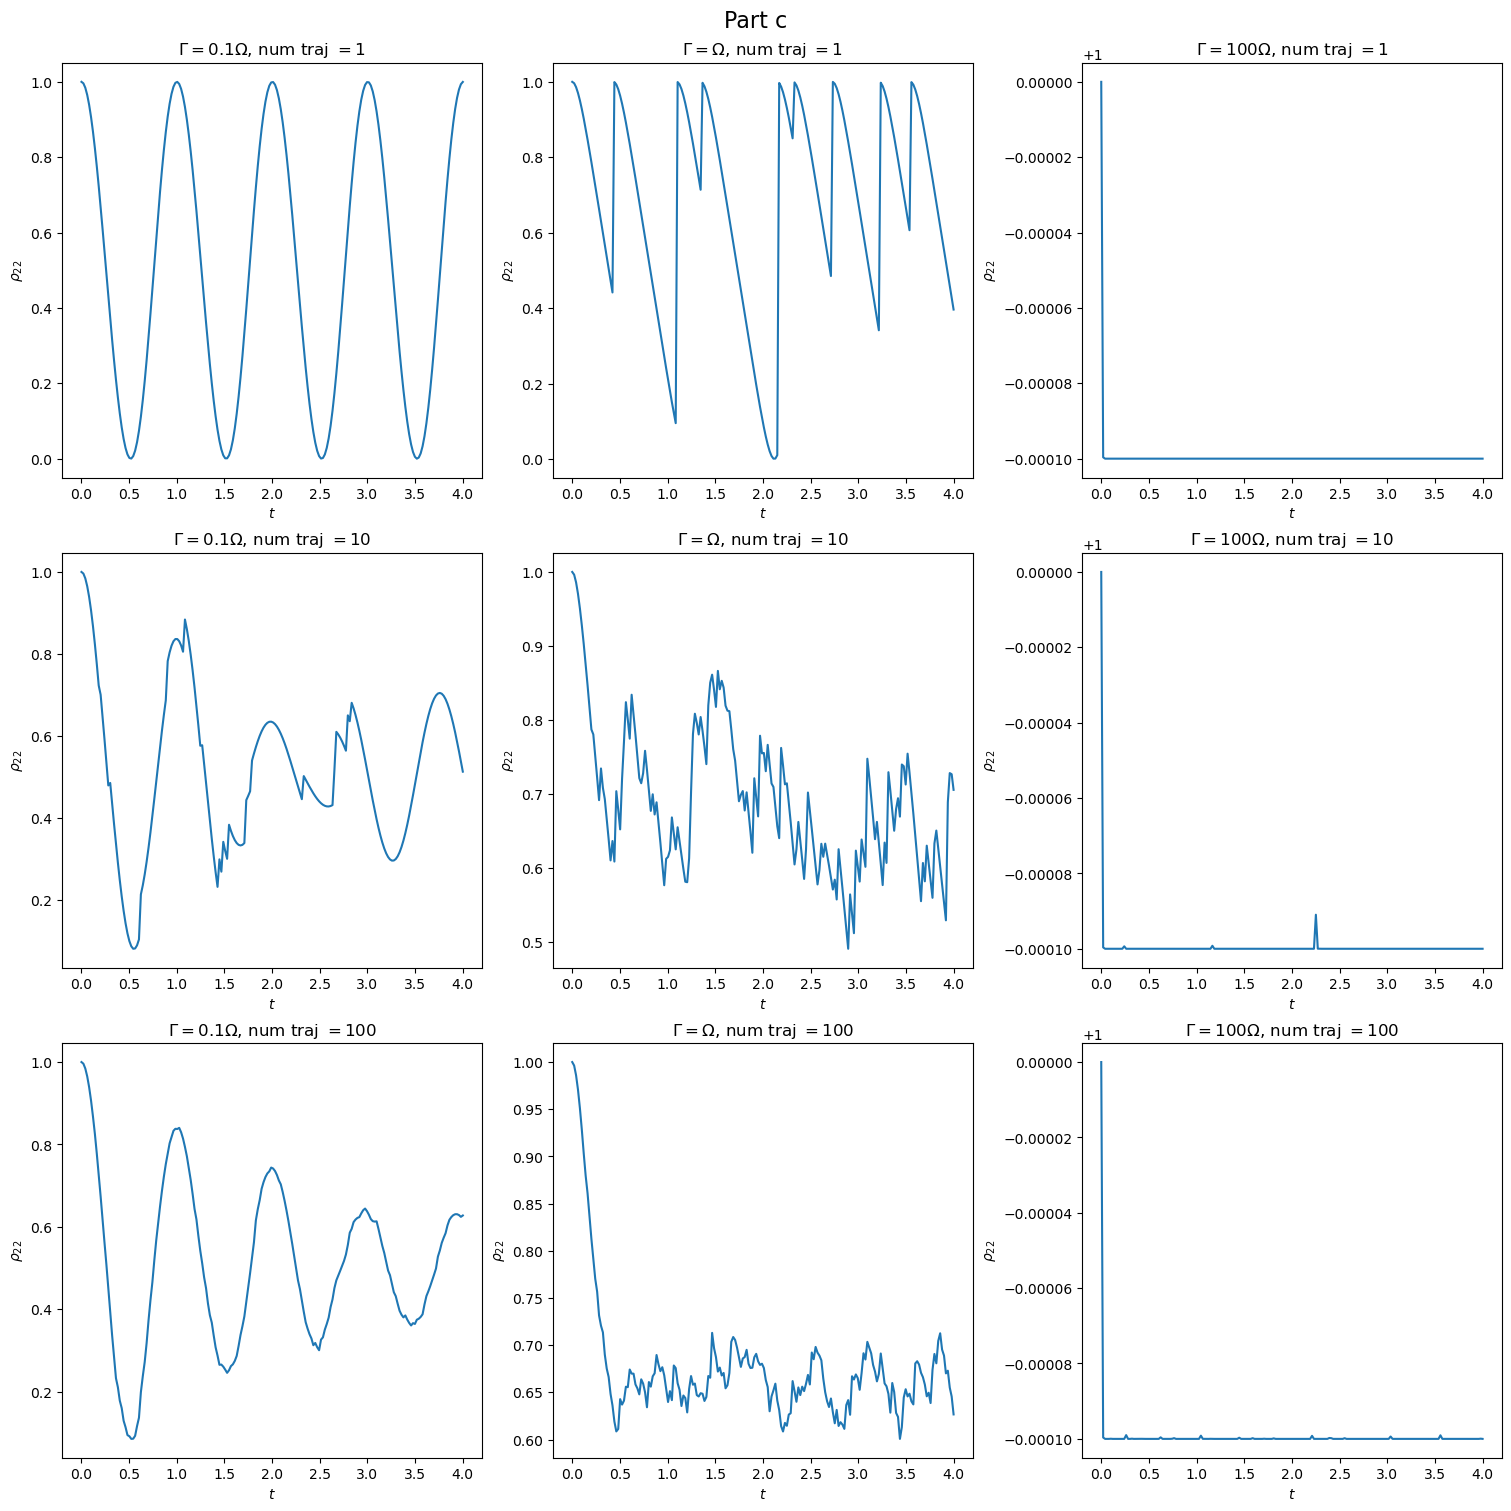
\includegraphics[width=1\linewidth]{Resources//245//Homework 9/245 Homework 9 Problem 5c.png}
    \label{fig:enter-label}
\end{figure}
\pagebreak
\section*{Code Appendix}
\section*{Problem 2}
\begin{python}
from qutip import ket, Bloch
from numpy import sqrt

psi = 1/sqrt(2)*(ket("0") + ket("1"))
rc = 1/sqrt(2)*(ket("0") + ket("1"))
rf = 0.7*rc

b = Bloch()

b.add_states(psi)
b.add_states(rc)
b.add_states(rf)

b.show()
\end{python}
\section*{Problem 5}
\subsection*{Part a}
\begin{python}
from numpy import pi, linspace, sqrt
from qutip import sigmax as sx
from qutip import sigmam as sm
from qutip import ket, mesolve, mcsolve
import matplotlib.pyplot as plt

# Hamilotnian
H = pi*sx()

# Assume we're in the pure initial state |1>
psi = ket("1")
rho = psi*psi.dag()

# Part a
ta = linspace(0,1,50)
def parta():
    rhoa = mesolve(H, rho, ta)
    return [r[1,1] for r in rhoa.states]

# Plot results
plt.close('all')

# Plot part a
fig1 = plt.figure(figsize=(5, 5), layout="constrained")
gs1_main = fig1.add_gridspec(1,1)

ax1 = fig1.add_subplot(gs1_main[0])
ax1.plot(ta,parta())
ax1.set_xlabel("$t$")
ax1.set_ylabel("$\\rho_{22}$")

fig1.suptitle('Part a', fontsize=16)
plt.show()
\end{python}
\subsection*{Part b}
\begin{python}
# Part b
Omega = 2*pi
tb = linspace(0,4,200)
def partb(Gamma):
    rhob = mesolve(H, rho, tb, c_ops=[sqrt(Gamma)*sm()])
    return [r[1,1] for r in rhob.states]
    
# Plot part b
fig2 = plt.figure(figsize=(15, 5), layout="constrained")
gs2_main = fig2.add_gridspec(1,3)

ax1 = fig2.add_subplot(gs2_main[0])
ax1.plot(tb,partb(0.1*Omega))
ax1.set_xlabel("$t$")
ax1.set_ylabel("$\\rho_{22}$")
ax1.set_title("$\\Gamma = 0.1\\Omega$")

ax2 = fig2.add_subplot(gs2_main[1])
ax2.plot(tb,partb(Omega))
ax2.set_xlabel("$t$")
ax2.set_ylabel("$\\rho_{22}$")
ax2.set_title("$\\Gamma = 10\\Omega$")

ax3 = fig2.add_subplot(gs2_main[2])
ax3.plot(tb,partb(3*Omega))
ax3.set_xlabel("$t$")
ax3.set_ylabel("$\\rho_{22}$")
ax3.set_title("$\\Gamma = 100\\Omega$")

fig2.suptitle('Part b', fontsize=16)
plt.show()
\end{python}
\subsection*{Part c}
\begin{python}
# Part c
def partc(Gamma, traj):
    rhoc = mcsolve(H, psi, tb, c_ops=[sqrt(Gamma)*sm()],ntraj=traj)
    return [r[1,1] for r in rhoc.states]
    
fig3 = plt.figure(figsize=(15,15), layout="constrained")
gs3_main = fig3.add_gridspec(3,3)

# 1 trajectory
ax1 = fig3.add_subplot(gs3_main[0])
ax1.plot(tb,partc(0.1*Omega,1))
ax1.set_xlabel("$t$")
ax1.set_ylabel("$\\rho_{22}$")
ax1.set_title("$\\Gamma = 0.1\\Omega$, num traj $= 1$")

ax2 = fig3.add_subplot(gs3_main[1])
ax2.plot(tb,partc(1*Omega,1))
ax2.set_xlabel("$t$")
ax2.set_ylabel("$\\rho_{22}$")
ax2.set_title("$\\Gamma = \\Omega$, num traj $= 1$")

ax3 = fig3.add_subplot(gs3_main[2])
ax3.plot(tb,partc(100*Omega,1))
ax3.set_xlabel("$t$")
ax3.set_ylabel("$\\rho_{22}$")
ax3.set_title("$\\Gamma = 100\\Omega$, num traj $= 1$")

# 10 trajectories
ax4 = fig3.add_subplot(gs3_main[3])
ax4.plot(tb,partc(0.1*Omega,10))
ax4.set_xlabel("$t$")
ax4.set_ylabel("$\\rho_{22}$")
ax4.set_title("$\\Gamma = 0.1\\Omega$, num traj $= 10$")

ax5 = fig3.add_subplot(gs3_main[4])
ax5.plot(tb,partc(1*Omega,10))
ax5.set_xlabel("$t$")
ax5.set_ylabel("$\\rho_{22}$")
ax5.set_title("$\\Gamma = \\Omega$, num traj $= 10$")

ax6 = fig3.add_subplot(gs3_main[5])
ax6.plot(tb,partc(100*Omega,10))
ax6.set_xlabel("$t$")
ax6.set_ylabel("$\\rho_{22}$")
ax6.set_title("$\\Gamma = 100\\Omega$, num traj $= 10$")

# 100 trajectories
ax7 = fig3.add_subplot(gs3_main[6])
ax7.plot(tb,partc(0.1*Omega,100))
ax7.set_xlabel("$t$")
ax7.set_ylabel("$\\rho_{22}$")
ax7.set_title("$\\Gamma = 0.1\\Omega$, num traj $= 100$")

ax8 = fig3.add_subplot(gs3_main[7])
ax8.plot(tb,partc(1*Omega,100))
ax8.set_xlabel("$t$")
ax8.set_ylabel("$\\rho_{22}$")
ax8.set_title("$\\Gamma = \\Omega$, num traj $= 100$")

ax9 = fig3.add_subplot(gs3_main[8])
ax9.plot(tb,partc(100*Omega,100))
ax9.set_xlabel("$t$")
ax9.set_ylabel("$\\rho_{22}$")
ax9.set_title("$\\Gamma = 100\\Omega$, num traj $= 100$")

fig3.suptitle('Part c', fontsize=16)
plt.show()
\end{python}